\documentclass{standalone}
\usepackage{tikz}
\usepackage{ctex,siunitx}
\setCJKmainfont{Noto Serif CJK SC}
\usepackage{tkz-euclide}
\usepackage{amsmath}
\usetikzlibrary{patterns, calc,3d}
\usetikzlibrary{decorations.pathmorphing,decorations.pathreplacing,decorations.shapes}
\begin{document}
\small
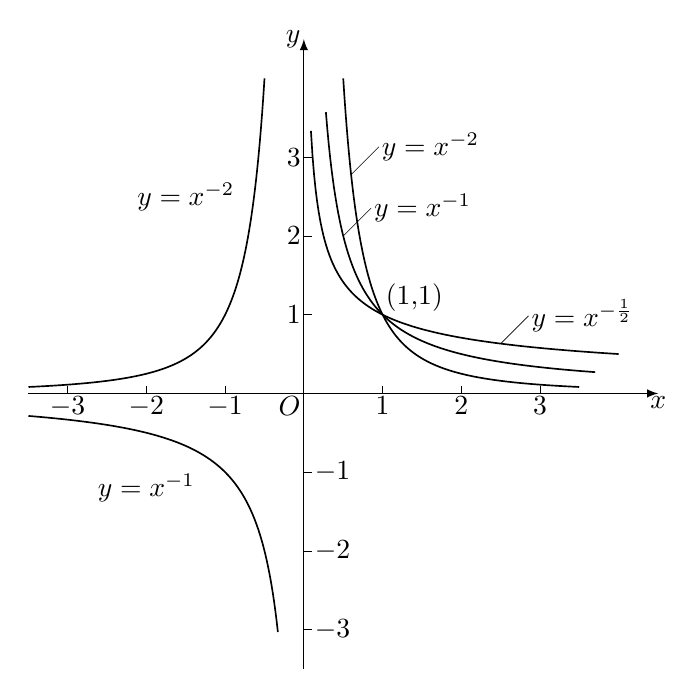
\begin{tikzpicture}[>=latex,scale=1.0,inner sep=1pt]
  \draw[->](-3.5,0)--(4.5,0)node[below]{$x$};
  \draw[->](0,-3.5)--(0,4.5)node[left]{$y$};
  \node at (0,0)[below left]{$O$};
  \draw[semithick,samples=200,domain=0.28:3.7]plot(\x,1/\x);
  \draw[semithick,samples=200,domain=0.09:4]plot(\x,{1/sqrt(\x)});
  \draw[semithick,samples=200,domain=-0.33:-3.5]plot(\x,1/\x);
  \draw[semithick,samples=200,domain=0.5:3.5]plot(\x,1/\x/\x);
  \draw[semithick,samples=200,domain=0.5:3.5]plot(-\x,1/\x/\x);
  \foreach \x in {1,2,3}
  {
    \draw[very thin](-\x,0)node[below]{$-\x$}--++(0,0.1);
    \draw[very thin](\x,0)node[below]{$\x$}--++(0,0.1);
    \draw[very thin](0,\x)node[left]{$\x$}--++(0.1,0);
    \draw[very thin](0,-\x)--++(0.1,0)node[right]{$-\x$};
  }
  \node at (-2,-1.2){$y=x^{-1}$};
  \node at (-1.5,2.5){$y=x^{-2}$};
  \node at (1,1)[above right]{(1,1)};
  \draw[very thin](0.5,2)--++(45:0.5)node[right]{$y=x^{-1}$};
  \draw[very thin](0.6,1/0.6/0.6)--++(45:0.5)node[right]{$y=x^{-2}$};
  \draw[very thin](2.5,0.632)--++(45:0.5)node[right]{$y=x^{-\frac12}$};
\end{tikzpicture}
\end{document}